\chapter{Implementation}
\label{prototype}

The \Meta\ prototype implements nodes, reductions, and grammars as described in the previous chapters, and a compiler for the kernel language. I built a core language via syntax extension of the kernel language. The \Meta\ editor is capable of editing and executing both grammars and core language programs.

\section{The Host Platform}
The prototype system is implemented in Clojure \cite{clojure}, a language in the Lisp family which runs on the Java Virtual Machine \cite{jvm}. Clojure also fills the role of the host kernel language. Some characteristics of Clojure that make it a good choice include:
\begin{enumerate}
\item Similar notion of a kernel language. The prototype simply adopts (a subset of) the special forms of Clojure as its kernel language.
\item Functional orientation. Clojure is a non-pure functional language; it allows side-effects but (in contrast to most Lisps) all of its bindings and data structures are immutable. %Destructive assignment is supported only for special \emp{reference} objects which enforce certain semantics (and which do not play any real role in this system). This approach fits quite well with the idea of transformation of immutable trees, and in fact inspired many ideas such as the approach to tree reduction.
\item Compilation service available at runtime. The Clojure compiler is part of the runtime stack, so once a program is reduced to the kernel language, it can be evaluated (compiled) and executed immediately.
\item Access to the Java platform. The prototype takes advantage of Java's GUI toolkit for rendering and editing.
%\item Compiles to Java bytecode, and allows direct access to the platform's objects when needed. For example, nodes are represented as instances of a class at the JVM level, which gives excellent performance with no representational overhead. It's some kind of triumph of compiler technology that a program in this system can achieve performance on par with raw C code. \todo{need to prove that?}
\end{enumerate}

Nodes are represented as a Lisp-style abstract data type comprising a series of functions \clojure{make-node}, \clojure{node?}, \clojure{node-type}, etc., which allow Clojure programs to construct and manipulate nodes independent of the concrete representation. The prototype uses only these functions to work with nodes.

The implementation of the node ADT uses Clojure's \clojure{deftype} construct to represent nodes as instances of a \clojure{nodetype} class at the JVM level. This reduces the overhead for simple nodes to the minimum. Map- and sequence-valued nodes use Clojure's built-in persistent hash map and persistent vector data structures (based on Bagwell's array mapped tries \cite{bagwell}) to store their children.

The \clojure{make-node} function provides a convenient serialized form for nodes: s-expressions. A \clojure{print-node} function turns a node object back into text which can be read and evaluated to re-constitute the node. This low-level representation is never seen by the user of the system.


\section{The Host Language}
\label{host}
The host language is composed of a kernel based on the primitive constructs and values of Clojure together with a core language built via syntax extension on top of the kernel language.

\subsection{The Kernel Language}
The kernel language, shown in Figure \ref{fig-kernel}, consists of six kinds of primitive values, six node types corresponding to Clojure's special forms, two nodes for quotation, and a node for making external references to the platform. Virtually every node is an instance of the abstract \keyword{expr} type, yielding some kind of value as a function of its arguments; there are no statements and no mutating assignments.

%The kernel language is somewhat simplified relative to the complete list of Clojure's special forms. A few forms which are not currently used are left out, and several of the nodes are somewhat less flexible in form than the corresponding Clojure syntax.

\begin{figure}
%  \todo{fix columns? clean up primitives with some syntax}
  
%  \fbox{
  \begin{minipage}[t]{0.48\linewidth}
  \vspace{0pt}  % align to top
  \begin{center}
  \includegraphics[scale=0.65]{src/image/kernel1.pdf}
  \end{center}
  \end{minipage}
%  }
%  \hfill
%  \fbox{
  \begin{minipage}[t]{0.48\linewidth}
  \vspace{0pt}  % align to top
  \begin{center}
  \includegraphics[scale=0.65]{src/image/kernel2.pdf}
  \end{center}
  \end{minipage}
%  }
  
%\todo{\keyword{loop}}

  \caption{\label{fig-kernel} Grammar for the host kernel language.}
\end{figure}

The kernel language is extremely simple compared to a typical general-purpose language. Like Clojure, the kernel language is not statically typed, which helps keep \Meta's implementation simple---all checking of operands is done at runtime, by the Clojure/Java platform. All but a few kernel language node types are instances of \keyword{expr}, representing expressions yielding a single value. This simplicity makes the language easy to implement, and makes it an easy target for reductions.

The primitive values of the kernel language are the singular values \keyword{nil}, \keyword{true}, and \keyword{false}, plus integers, strings, and names.

A \keyword{lambda} node introduces a function taking a fixed number of arguments. A \keyword{params} node always represents the parameters of a function, and can appear only as the \keyword{params} attribute of a \keyword{lambda} node. Each parameter is a \keyword{bind} node, discussed later. A lambda node is ``bound'' within its body, supporting simple recursive calls. \keyword{recur} is a non-stack-consuming recursive call, and must appear in tail position.

$n$-ary functions are included in the kernel language as they are in Clojure to allow a simple mapping to Java methods for high performance without sophisticated compilation techniques. The kernel language does not support Clojure's variable-arity functions.

\keyword{app} is (call-by-value) function application. The \emp{expr} is evaluated first (to a function), then the expressions in \keyword{args} are evaluated from left to right. 

Simple conditionals are provided by \keyword{if}. All values except \keyword{false} and \keyword{nil} are treated as true when they appear as the \emp{test} expression.

\keyword{let} evaluates an expression, binds a name to the resulting value and then evaluates its body with that binding in scope. \Meta\ provides only a single-binding, non-recursive primitive \emp{let} form.

A \keyword{var} node is a reference to the value bound by the parameter of a lambda, by the lambda itself, or by a let expression. Variables are lexically-scoped, and lambdas capture all bindings in scope at their point of declaration. All these forms are strict in all their arguments, and have no side-effects.

An \keyword{extern} node refers to a variable at the Clojure level. This allows any function or value defined by the Clojure platform or \Meta\ runtime to be accessed. Use of these external facilities is minimized in order to make the core language as self-contained as possible.

\keyword{quote} and \keyword{unquote} are given special treatment by the meta-compiler.


\subsection{Meta-compilation}
Given a program in the kernel language, a function \clojure{meta-compile} translates the nodes to Clojure s-expressions in a mostly straight-forward way, due to the close correspondence between kernel nodes and Clojure's special forms. Only a few types of nodes need special consideration. %Then Clojure's \clojure{eval} function is invoked, and the program is compiled to Java bytecode, loaded into the JVM, and executed. Because the kernel language maps so closely to Clojure's forms, the meta-compilation process is mostly trivial.

%Each kernel language node corresponds precisely to a Clojure special form or value, without any additional interpretation. Furthermore the structure of a Clojure program after reading matches the structure of the kernel program precisely: a Clojure program is a tree made from lists where the first element of each list is a symbol which names a special form. For example, the list produced by the reader for the string \clojure{"(+ 1 (* 2 3))"} has exactly the same overall shape as the corresponding kernel language program, with lists replaced by \keyword{app} nodes, and the simple names \clojure{*} and \clojure{+} wrapped in \keyword{extern} nodes. \todo{include a picture of the nodes version? How to do that without going into presentation issues? Can I avoid having tons of pictures of trees?}

A \keyword{bind} node is reduced to a symbol, and a \keyword{var} node to the symbol of the corresponding binding. The problem of producing suitable names and avoiding conflicts is easily solved due to the uniqueness of labels in the \Meta\ program. The meta-compiler simply generates a new name for each label and uses that name for both \keyword{bind} and \keyword{var} nodes.

When the meta-compiler encounters a \keyword{quote} node, it enters a separate mode where instead of translating kernel language nodes to s-expressions, it instead translates nodes (potentially in any language) to s-expressions that construct a new copy of the quoted nodes. When an \keyword{unquote} node is encountered, the meta-compiler reduces the contents in the normal way, and then inserts the resulting value into the expression building the quoted node. Quotations may be nested more than one level deep, so the reduction keeps track of the current level and only resumes ordinary translation when the level reaches zero.

When quoted nodes are compiled, they are relabeled (that is, each node is assigned a fresh, globally-unique label) and each non-free reference is updated to point to the new node. This is important because it means that no code outside of the newly-generated fragment can possibly contain a reference to anything defined in it. For example, reductions for syntax extensions commonly bind values to names (in order to control evaluation order, for example), and each name is defined by some \keyword{bind} node. So in a reduced program, each instance of the reduced fragment will contain a binding which originated in the same node, but each binding is completely distinct and independent in the reduced program due to the relabeling that is performed when the reduction is executed. Because all names are unique at all times, the problem of ``hygienic macros''\cite{hygiene} does not arise.

Once a kernel language program has been meta-compiled, the standard Clojure function \clojure{eval} is invoked, which compiles the expression to Java bytecode, loads it into the running JVM, invokes it, and returns the result as a Clojure/Java value. %When necessary a function is available to ``wrap'' that value in (kernel language) nodes which represent the same value. This \emp{unread} mechanism will be discussed later. \todo{Will it? Come back to these implementation details later or not?}


\subsection{Core Language}
The host core language provides common facilities built via syntax extension on top of the kernel language. 
%That is, nodes of the core language are reduced to kernel language nodes prior to meta-compilation. 
A subset of Clojure's Core API~\cite{clojure-and} is implemented, plus primitives for constructing and manipulating AST nodes. Some examples using the syntax which exposes Clojure's cons-list primitive are shown in Figure~\ref{fig-core}. Some of the definitions used in these examples are presented in Section~\ref{for}.

%One such primitive is \keyword{cons} (rendered as an infix `:'), which constructs a lazy sequence given head and tail expressions; the head is evaluated immediately, and the tail expression is wrapped in a thunk---it will be evaluated the first time the tail of the resulting sequence is needed. This simple mechanism allows lazy infinite sequences to be used in core language programs, as seen in some of the examples in Figure \ref{fig-core}.

\begin{figure}	
	\centering

	\includegraphics[scale=0.8]{src/image/core3.pdf}
	
	\caption{Example core language expressions and their values.}
	\label{fig-core}
\end{figure}

%\todo{some more examples and/or some of the grammar?}


\subsection{Compiling Reductions}
To employ a \emp{display} or \emp{expand} reduction defined in a grammar, it needs to be transformed into a reduction function which can be applied to a source program node, yielding a reduced node (see Section~\ref{reduction}). Each reduction in the grammar is an expression which may contain variables referring to the attributes of the node. Therefore a reduction function can be constructed by simply wrapping the reduction expression in a lambda abstraction and a series of \keyword{let}s binding each of the attributes. For example, the reduction for \keyword{string} nodes looks like this:
\begin{center}
\includegraphics{src/image/reduce.pdf}
\end{center}
where $\keyword{attr}[\mathit{node}, \mathit{name}]$ extracts the named attribute from a node. Once the \keyword{value} attribute is bound, the result node is constructed by evaluating the quoted \keyword{string} node (which appeared in the actual declaration in the grammar shown in Figure~\ref{fig-kernel}).

A similar function is constructed and compiled for each node type, and then an overall reduction function is built which dispatches to the right reduction based on the type of each node. This overall function is built incrementally as the declarations of a grammar are processed, so that later reductions can make use of syntax defined in earlier declarations.

%
% Rendering :expr:
%
\section{Rendering the Expression Language}

After a program is reduced to the \keyword{expr} presentation language (via the \keyword{display} reductions specified in the particular grammar being used), it can be presented to the user using the common facilities of \Meta. To do so, the program is further reduced to a low-level presentation language.


\subsection{The \textit{\keyword{view}} Presentation Language}
\label{view}

The \keyword{view} language is a lower-level presentation language. Some of the algorithms of \TeX\ \cite{tex-math} are used to lay out nodes and construct glyphs, as in e.g.\ \cite{mathml}. In contrast to the \keyword{expr} language, all the elements of the \keyword{view} language specify fonts, colors, and sizes in concrete terms, so they can be rendered directly. The main tasks of the reduction from \keyword{expr} to \keyword{view} are to identify the correct font size for each atom based on the nesting of expressions, and to transform \keyword{embed}/\keyword{disembed} nodes into border/background colors. Both of these computations involve propagating some information about the structure of the tree down as the nodes are recursively processed.

The mode, a concept from \TeX, identifies the depth of nesting of expressions, and controls the selection of font sizes for atoms. There are four modes, \textit{Display} ($D$), \textit{Text} ($T$), \textit{Script} ($S$), and \textit{Scriptscript} ($SS$). $D$ and $T$ call for normal-sized text, $S$ is about 30\% smaller, and $SS$ is about 50\% smaller.The handling of modes follows \TeX's algorithm in most cases, but deviates from it when necessary for consistency. For example, typographical convention dictates that addition expressions in the smaller modes should be set without spaces, but that would clash with \Meta's handling of parentheses, so \Meta\ sets these expressions with proportionately smaller spaces.

Each of the atom types of the \keyword{expr} language is reduced to a \keyword{chars} node. For example, when a node $n$ having the type \keyword{keyword} and \emp{str} attribute $s$ is reduced:
$$
n:~\mapnode{keyword}{ \attr{str}{s} } 
 	\reduces
	\mapnode{chars}{ \attr{str}{s},~\attr{font}{ \mathbf{keywordfont}_{\mathbf{mode}[n]}} }
$$
where $\mathbf{keywordfont}_D$ and $\mathbf{keywordfont}_T$ are both names for the normal-size font for keywords, and $\mathbf{keywordfont}_S$ and $\mathbf{keywordfont}_{SS}$ name the two smaller versions. $\mathbf{mode}[n]$ is an inherited attribute~\cite{attribute-grammar}; except where specified, the mode of each node is the mode of its parent. Except for a handful of types, most atoms are reduced in exactly the same way, with a different font used for each type.

\vspace{12pt}
% string -> chars
Atoms representing string literals get special treatment. They're surrounded by quotes, and any white space characters in the string value are replaced by Unicode OPEN BOX characters (~\textvisiblespace~).
$$
n:~\mapnode{string}{\attr{str}{s}} 
 	\reduces
	\mapnode{chars}{\attr{str}{\textrm{``} + \mathbf{escapewhitespace}[s] + \textrm{''}},
		~\attr{font}{\mathbf{stringfont}_{\mathbf{mode}[n]}} }
$$

\vspace{12pt}
% -> sequence
Each of \keyword{expr}'s four sequence types are reduced to a single type, and spaces are inserted between the child nodes:
\begin{align*}
& \seqnode{juxt}{ c_0, c_1, \dots, c_m }
 	\reduces
	 \seqnode{sequence}{ c_0, c_1, \dots, c_m }
\\
& \seqnode{binary}{ c_0, c_1, \dots, c_m }
 	\reduces
	 \seqnode{sequence}{ c_0, \keyword{thinspace}, c_1, \keyword{thinspace}, \dots,\keyword{thinspace}, c_m }
\\
& \seqnode{relation}{ c_0, c_1, \dots, c_m }
 	\reduces
	 \seqnode{sequence}{ c_0, \keyword{mediumspace}, c_1, \keyword{mediumspace}, \dots,\keyword{mediumspace}, c_m }
\\
& \seqnode{flow}{ c_0, c_1, \dots, c_m }
 	\reduces
	 \seqnode{sequence}{ c_0, \keyword{thickspace}, c_1, \keyword{thickspace}, \dots,\keyword{thickspace}, c_m }
\end{align*}


\vspace{12pt}
% fraction -> over
A \keyword{fraction} node is reduced to \keyword{over}, which has a configurable line weight, and the mode of each child is reduced:
$$
n: \mapnode{fraction}{ \attr{numer}{c_0},~\attr{denom}{c_1} } 
 	\reduces
	\mapnode{over}{ \attr{top}{c_0},~\attr{bottom}{c_1},~\attr{weight}{1} }
$$
\begin{align*}
\mathbf{mode}[c_0] & \leftarrow \mathit{fractionmode}(\mathbf{mode}[n])
\\
\mathbf{mode}[c_1] & \leftarrow \mathit{fractionmode}(\mathbf{mode}[n])
\end{align*}
\begin{align*}
\mathit{fractionmode}(D) & = T
\\
\mathit{fractionmode}(T) & = S
\\
\mathit{fractionmode}(S) & = SS
\\
\mathit{fractionmode}(SS) & = SS
\end{align*}

\vspace{12pt}
% scripted
A \keyword{scripted} node is unchanged except that the mode of the raised and lowered child nodes is reduced:
$$
n: \mapnode{scripted}{ \attr{nucleus}{c_0},~ 
							\attr{super}{c_1},~
							\attr{sub}{c_2} } 
$$
\begin{align*}
\mathbf{mode}[c_1] &\leftarrow \mathit{scriptmode}(\mathbf{mode}[n])
\\
\mathbf{mode}[c_2] &\leftarrow \mathit{scriptmode}(\mathbf{mode}[n])
\end{align*}
\begin{align*}
\mathit{scriptmode}(D) &= S
\\
\mathit{scriptmode}(T) &= S
\\
\mathit{scriptmode}(S) &= SS
\\
\mathit{scriptmode}(SS) &= SS
\end{align*}

\vspace{12pt}
% embed -> border
The \keyword{embed} and \keyword{disembed} nodes which represent quotations and other kinds of embedded code are reduced to \keyword{border} nodes, which draw a colored border around their contents and a background behind them. The color of each border is determined by the meta-level of the node. The level of the root node is always 0, and it is incremented when an \keyword{embed} node is encountered:
\begin{align*}
n:~& \mapnode{embed}{ \attr{content}{c} }
\\
	& \to 
	\mapnode{border}{\attr{weight}{1},~
					\attr{margin}{3},~ 
					\attr{border}{b},~ 
					\attr{fill}{f},~ 
					\attr{content}{c} }
\end{align*}
\begin{align*}
b &= \mathbf{bordercolor}_{\mathbf{level}[c]}
\\
f &= \mathbf{fillcolor}_{\mathbf{level}[c]}
\end{align*}
\begin{align*}
\mathbf{level}[c] & \leftarrow \mathbf{level}[n] + 1
\end{align*}
Two series of colors $\mathbf{bordercolor}_i$ and $\mathbf{fillcolor}_i$ are pre-defined. $\mathbf{bordercolor}_1$ is dark blue, $\mathbf{bordercolor}_2$ is dark green, etc. Six colors are defined to support several levels of embedding. $\mathbf{fillcolor}_0$ is white (the background color of ordinary nodes). $\mathbf{fillcolor}_i$ is a lighter shade of $\mathbf{bordercolor}_i$.

For \keyword{disembed}, a similar border, but the border color corresponds to the \emp{parent} node's meta-level, while the background indicates the level of the inner node:
\begin{align*}
n:~& \mapnode{disembed}{ \attr{content}{c}, \attr{levels}{l} }
\\
	& \to 
	\mapnode{border}{\attr{weight}{1},~
					\attr{margin}{3},~ 
					\attr{border}{b},~ 
					\attr{fill}{f},~ 
					\attr{content}{c} }
\end{align*}
\begin{align*}
b &= \mathbf{bordercolor}_{\mathbf{level}[n]}
\\
f &= \mathbf{fillcolor}_{\mathbf{level}[c]}
\end{align*}
\begin{align*}
\mathbf{level}[c] & \leftarrow \mathbf{level}[n] - l
\end{align*}

\vspace{12pt}
The remaining nodes of the \keyword{expr} language require no special handling, because they do not affect the mode or meta-level of their sub-expressions.

A handful of additional nodes are provided in \keyword{view} for handling some of the needs beyond what \keyword{expr} can do. A \keyword{section} arranges its children in a left-aligned vertical stack. A wider space node, \keyword{quad}, is useful for indentation.

The reduction described in this section is implemented directly in Clojure, not in a \Meta\ grammar, because the grammar language does not currently provide any way to declare attributes. That might be a useful extension; if both inherited and synthesized attributes \cite{attribute-grammar} could be defined, it would be possible to write type systems for expressions. However, the burden of implementing this particular reduction manually is modest because the \keyword{expr} language is small and not meant to be extended.

The smaller modes quickly become hard to read for anything but very simple expressions (especially on relatively low-resolution displays), so wise language designers (and programmers) will use them sparingly. The \TeX book \cite{knuth} gives much good advice about how to use them effectively. Some clear applications of the smaller modes are for constant ratios and exponents, and for decorating variable names with small integer subscripts and ``prime'' symbols, as in $x' = \frac{1}{2}x^2 + a_0$.


\subsection{Rendering the \textit{\keyword{view}} Presentation Language}
The \keyword{view} language is consumed by a \emp{renderer} written in Clojure using the graphics primitives of Java2D \cite{java2d}. The renderer recursively inspects the tree, calculating node sizes and layout, and then actually drawing nodes. The renderer also provides hit-testing for nodes, identifying a list of \keyword{view} nodes which enclose a given point.

For each node, the renderer calculates a width $w$ and height $h$ in (floating-point) pixels. Depending on the node type, there may be a baseline height, $b$ (between 0 and $h$), which defines the position of the node relative to a common baseline. When a node has children, the renderer calculates a horizontal and vertical position $(x, y)$ for each child, relative to the upper-left corner of the parent node.

For \keyword{chars} nodes, $w$, $h$, and $b$ values are calculated based on the string and font via Java2D. In general, other nodes' baselines are derived from their children, so that the \keyword{chars} nodes in nearby parts of the tree are baseline-aligned.

In a \keyword{sequence}, child nodes with baselines are vertically aligned to their baselines, and children without baselines are aligned to their centers (and to the collective center of the baseline-aligned nodes).

The baseline of a \keyword{scripted} node is that of its nucleus. An \keyword{over} node has no baseline. 

The delimiters of a \keyword{group} node (e.g. parentheses or brackets) are vertically centered relative to the contents, and the actual glyph is chosen from a list of variously-sized alternatives. \TeX's fonts are used for these glyphs, as well as for most symbols reduced from \keyword{expr/symbol}.

Any node can have a \keyword{color} attribute, which causes the single node to be drawn with a different foreground color.

These definitions are sufficient to get simple expressions to render well, but the current algorithm lacks \TeX's second alignment step (the \emp{axis}), so some expressions are not quite properly aligned (e.g. fraction lines are not aligned with the vertical centers of $+$ and $-$ operators).


%Size and layout are calculated as follows:
%\begin{eqnarray*}
%w & = & \sum w_i
%\\
%h & = & \mathrm{max}\left( h_b, \mathrm{max}(h_i) \right)
%\\
%b & = & (h/2 - h_b/2) + a_\mathrm{max}
%\\
%x_i & = & \sum_{j=0}^{i-1} w_i 
%\\
%y_i & = & \left\{
%		\begin{array}{lr}
%			b - b_i, & b_i\ \mathrm{defined}
%			\\
%			(h - h_i)/2, & \mathrm{otherwise}
%		\end{array}
%		\right.
%\\
%where &
%\\
%h_b & = & a_\mathrm{max} + d_\mathrm{max},\ \textit{the aggregate height of baseline-aligned nodes}
%\\
%a_\mathrm{max} & = & \mathrm{max}(b_i),\ \textit{the largest ascent}
%\\
%d_\mathrm{max} & = & \mathrm{max}(h_i - b_i),\ \textit{the largest descent}
%\end{eqnarray*}

%A \keyword{section} node contains a vertical series of nodes aligned at their left edges:
%\begin{eqnarray*}
%w_\mathrm{section} & = & \mathrm{max}(w_i)
%\\
%h_\mathrm{section} & = & \sum h_i
%\\
%b_\mathrm{section} & = & b_0
%\\
%x_i & = & 0
%\\
%y_i & = & \sum_{j=0}^{i-1} h_i
%\end{eqnarray*}


%\keyword{over}, \keyword{radical}, and \keyword{delimited} nodes were described earlier. \keyword{border} draws its content with a background color, surrounded by a rectangular border with a configurable weight.

%For layout purposes, the renderer calculates a size for each node, consisting of width, height, and optional baseline height. A baseline is calculated for each \keyword{chars} node based on its font, and certain other nodes calculate a baseline based on their contents. \keyword{sequence} nodes' children are laid out so that nodes with baseline heights are aligned to a mutual baseline, and nodes without baseline heights are aligned to their vertical center (and the overall vertical center of all baseline-aligned siblings). This is sufficient to get simple expressions to render well, but the current algorithm lacks \TeX's second alignment step (the \emp{axis}), so some expressions are not quite properly aligned (e.g. fraction lines are not aligned with the vertical centers of $+$ and $-$ operators).
 
%\keyword{radical} and \keyword{delimited} nodes are laid out by first sizing the content node, then selecting the appropriate glyph(s) from a list of variously-sized alternatives, and finally calculating sizes and positions based on the selected glyph. \TeX's fonts are used for these glyphs, as well as for most symbols reduced from \keyword{expr/symbol}. 

The renderer makes several passes over the tree to draw different layers. The first pass draws only \keyword{border} nodes, which therefore appear ``behind'' all other elements. The nodes are drawn in pre-order, so that parent borders and their background fill are drawn behind any child borders. On the second pass, an indicator of the selected node is drawn, so that it will appear above the border rects, but behind the actual content. The final pass renders all non-border nodes.


\subsection{Renderer Implementation}

The renderer is written in a simple functional style, freely traversing the node tree as much as necessary. However because some of the necessary calculations are relatively expensive, the renderer initially performed poorly, taking on the order of 2-500ms to render a small program. This was easily improved by taking advantage of the fact that much of the renderer's time is spent in two kinds of referentially-transparent functions. The function that calculates the size of a text glyph given the characters and font is simply memo-ized, so that no more than one call is ever made for each unique glyph. The functions that calculate the position of each node are also cached, but only for the duration of a single rendering pass (mostly to avoid consuming arbitrary memory for no-longer-needed cached values when a succession of updated trees is rendered one after the other). That way the renderer performs well (10-20ms) despite being written in the most direct way, making no attempt to avoid redundant calculations. Clojure's functional nature and macro facility made it easy to implement this algorithmic change ``after the fact,'' without requiring the bulk of the rendering code to be re-written.

The renderer currently violates good functional programming style by performing the actual drawing via side-effecting operations during the traversal of the node tree. In hindsight, it would have been better to have the traversal yield a list of drawing commands to be executed later. For instance the layering of different kinds of visual elements could have been handled declaratively, rather than as a side-effect of traversal order.


%\subsection{Reducing \textit{\keyword{expr}} to \textit{\keyword{view}}}
%The reduction from \keyword{expr} to \keyword{view} is the most complex in \Meta, because it involves some non-local information. It is written by hand using an enhanced reduction algorithm which keeps track of a pair of values at each node: \emp{display mode} and \emp{meta-level}.

%The mode, a concept from \TeX, identifies the depth of nesting of expressions, and controls the selection of font sizes for atoms. There are four modes, \textit{Display} ($D$), \textit{Text} ($T$), \textit{Script} ($S$), and \textit{Scriptscript} ($SS$). By default, the mode of the root node is $T$, and the mode is decreased (roughly in sequence) whenever notational convention dictates that subexpressions should be typeset in a smaller font. When reducing an atom, the atom type and mode are used to look up the appropriate font. The handling of modes follows \TeX's algorithm in most cases, but deviates from it when necessary for consistency. For example, typographical convention dictates that addition expressions in the smaller modes should be set without spaces, but that would clash with \Meta's handling of parentheses, so \Meta\ sets these expressions with proportionately smaller spaces.

%\begin{figure}[h]
%\begin{center}
%\todo{capture something real}
%\end{center}

%$$
%\mathrm{D:} \quad
%a + b^2 + x^{c_1}
% - { x^{i+1} \over y }
% + { 1 \over { 1 \over R_1 }
% + { 1 \over R_2} }
% - \left({ 1 \over R_1 } + { 1 \over R_2}\right)^{-1}
%$$

%$$
%\mathrm{T:} \quad
%\textstyle
%a + b^2 + x^{c_1}
% - { x^{i+1} \over y }
% + { 1 \over { 1 \over R_1 }
% + { 1 \over R_2} }
% - \left({ 1 \over R_1 } + { 1 \over R_2}\right)^{-1}
%$$
%\caption{\label{fig-modes} Program fragment with multiple modes.}
%\end{figure}

%As the example in Figure \ref{fig-modes} shows, the smaller modes quickly become hard to read for anything but very simple expressions (especially on relatively low-resolution displays), so wise language designers (and programmers) will use them sparingly. The \TeX book\cite{knuth} gives much good advice about how to use them effectively. One clear application of the smaller modes in ordinary programs is for decorating variable names with small integer subscripts and ``prime'' symbols, as in $x' = x + a_0$.

%The meta-level is a non-negative integer indicating the level of nesting of the current node. It begins at zero and is incremented whenever an \keyword{embed} node is encountered and decremented on \keyword{disembed}. The \keyword{embed} node itself is reduced to a \keyword{border} which draws a light-colored background behind the embedded nodes, and a darker border of the same hue. A \keyword{disembed} node becomes a border with the hue of the lower level and the background of the outer level, making a visual connection between the outer and nested nodes that are at the same level. A fixed series of colors is used that can unambiguously indicate nesting of up to a half-dozen levels. An example of multi-level embedding appears in Figure \ref{fig-binary}, where the declaration is at level 0 (white background). The embedded right-side reduction is at level 1 (blue background), and it in turn contains a pair of embedded reductions (level 2, green background). The \emp{left} and \emp{right} attributes of the inner declaration are un-quoted (dis-embedded) back to level 1 within the level-2 reductions, while the \emp{op} and \emp{fn} are un-quoted to level 0.

%To compute the mode and meta-level at each node, the reduction function is extended to take the two values as additional parameters, and to return the pair of values along with the reduced node each time it is invoked. As the tree is visited, the values that were computed for a given node are passed to the reduction for its children. This allows the reduction function to compute values based on the shape of the tree, which would otherwise be impossible due to the lack of any reference from a sub-tree to its parent node. Effectively, the ``inherited'' value allows the reduction function to accumulate some information about the otherwise inaccessible ancestors. This simple extension is sufficient for this reduction (the most complicated yet encountered), and it does mean that this reduction could not be implemented in a grammar as almost all other reductions in \Meta\ are. A more sophisticated grammar language could support this kind of reduction, perhaps represented as an attribute grammar.\cite{attribute-grammar}


\subsection{Meta-reduction of \textit{\keyword{expr}}}
When editing regular programs, the \keyword{expr} language is meant to be invisible. When editing a grammar, the \keyword{expr} nodes of each presentation reduction are the subject at hand, so it's necessary for understanding to make them visible. To accomplish this, another hand-written reduction is used when editing grammars. This reduction decorates each node with a visual indication of its type, location, and size. This reduction is somewhat idiosyncratic in that it never actually replaces a node, but rather it inserts additional nodes (super-scripted \keyword{border} nodes), which surround the original nodes. Also, this reduction needs to be restricted to operate only on \keyword{expr} nodes of the original program, and not any nodes that might have been introduced by a reduction that was applied earlier. The reduction function is wrapped in a higher-order function that tracks which nodes remain to be reduced, using the mechanism described in the previous section.

The result can be seen in any of the examples of presentation reductions presented earlier. The idea of using a higher-order function (combinator) to assemble multiple simple reductions into something more complex came up again and again in building the prototype.


\subsection{Fallback Presentation Reduction}
Another useful reduction is one that is able to reduce any arbitrary node, imposing no restrictions whatsoever on the type or value of the node. This reduction can be used to show the internal structure of a node, disregarding the presentation reduction, or for displaying nodes for which no presentation reduction is available. This might be because the node's type is not declared in any applicable grammar, or because the presentation reduction itself is missing or unusable. All of these scenarios represent situations that \Meta\ aims to handle gracefully, because all of them can arise in the process of editing a program and/or the grammar that defines its language.

The solution is a \emp{fallback reduction}, which takes any node and reduces it to a node in the \keyword{view} language. A primitive-valued node is shown with a default style (similar to \keyword{expr}'s int, string, or name). A map- or sequence-valued node is surrounded by a border to set off the node as special, with the node type at the top and a series of lines with the attributes/indices and their values.

\begin{figure}[t]
  \begin{center}
  \includegraphics{src/image/gen.pdf}
  \end{center}
  \caption{Program fragment using a \keyword{cube} node, which hasn't been defined.}
  \label{fig-general}
\end{figure}

In Figure \ref{fig-general}, the programmer has attempted to write 
$3  + (1 + 2)^3$, 
but has used a ``cube'' node type for which no reduction is present. The fallback reduction makes the structure of the program clear in the absence of any specific knowledge of the ``cube'' node type, and gives the programmer the information she needs to figure out how to fix it. In this case she can either add a declaration for ``cube'' or change the program to use a different node type. This implementation does a good job of drawing attention to nodes that aren't handled properly and thus need attention, but it may be overly jarring when used within the context of an otherwise valid expression. Therefore, there may be a role for a less obtrusive reduction which shows any properly-defined children and gives an indication that something is amiss.


%
% Editing
%
\section{Editing}
The \Meta\ editor assembles the components described in the previous sections, along with a GUI shell. Each program is displayed in a separate window within a single process. When a grammar is used in the rendering of a program, changes to the grammar are reflected in the program's display immediately. Grammars and other kind of programs are presented and edited in the same way, the only difference being that a different sequence of reductions is applied. Neither the UI nor the programs themselves currently provide any way to specify the reductions that are to be applied to a particular program; it's up to the user to do that when invoking the editor.

An editor window (see Figure\ \ref{fig-editor}) shows a program in a scrollable panel, accompanied by some additional information about the selected node, if any. Actions to edit the program are available in the menus, or via keystrokes.

\begin{figure}[t]
	\centering
  
	\includegraphics[scale=0.60]{src/image/editor.png}
  
	\caption{The \Meta\ editor, showing a portion of the grammar for the core language.}
	\label{fig-editor}
\end{figure}


\subsection{Editor Pipeline}
To convert a program into \keyword{view} nodes for rendering, the editor applies a series of reductions in turn, as diagrammed in Figure~\ref{fig-pipeline}. Some of the reductions are baked into the platform, while others are compiled at runtime from the grammars that are specified when the editor is invoked. The first set of reductions takes different program elements from the source language to the \keyword{expr} language. A special reduction handles names, and another introduces a \keyword{missing} node wherever the grammar in effect defines an attribute (even if optional) but the program doesn't actually contain such a node. Then the reduction defined by the grammar is applied. At this point, all language-specific syntax should have been replaced by \keyword{expr} nodes, if the program and grammar are correct.

Next, a pair of reductions produce the final \keyword{expr} program, inserting parentheses where they are needed, and reducing any remaining non-\keyword{expr} nodes in the generic way. Next the \keyword{expr}-to-\keyword{view} reduction reduces the program to the \keyword{view} nodes that will be rendered, and finally that program is handed to the renderer for layout and drawing.

\begin{figure}[t]
	\begin{center}
	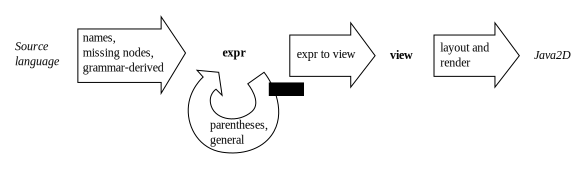
\includegraphics[scale=0.8]{src/image/pipeline.pdf}	
	\end{center}

	\caption{Reductions in the editor pipeline.}
	\label{fig-pipeline} 
\end{figure}

The editor itself takes charge of executing the reductions, keeping track of how the final \keyword{view} nodes were derived from the source program. Thus the end product of the rendering pipeline is a target program in the \keyword{view} language, plus a map identifying the target program node that arose from each source program node. Because a source program node often reduces to a sub-tree rather than a single node, not every target program node is identified with a source; only the root of each sub-tree needs to be tracked. The editor uses this tracking of nodes to let the user interact with the nodes of the \emp{source} program, even though what's actually being rendered is the target program, many layers of reduction removed.

%When it's desirable to keep track of what source node gave rise to a given target node, the reduction can record the labels of each pair of source and target node, forming a kind of mapping between the parallel trees. 

The need to map target nodes back to source nodes drove many decisions about how to represent programs. The presentation reduction must operate on one node at a time, and must produce a single target node. For example, the arguments of an \keyword{app} node are held by a characteristic \keyword{args} node mostly so that the editor can identify the resulting sequence of nodes and provide appropriate editing actions on them. For now, \keyword{expand} reductions are not so restricted, because \Meta\ does not try to trace nodes of reduced programs back to the corresponding source node. However, that might become desirable in the future, for instance in order to provide proper source locations for runtime errors.

%\temp{For this to work, the reduction function needs to operate strictly on the single node it's given, and not reach into any child node. This in turn places some constraints on the way the source program is constructed: each node (along with any environment) must bear sufficient information to identify the correct reduction.}


\subsection{Selection}
One of the main tasks of the editor is to make the structure of the program apparent to the programmer. Rendering the nodes of the program in a rich, familiar notation enhances readability but may not always make the structure of nodes very clear. In order to make a change to the AST, the programmer needs to be aware of this structure. The editor's UI for selection facilitates this awareness by visually emphasizing the relationship between a single selected node and its children, and by providing a way to move between nodes that is defined in terms of the source AST. Thus the structure becomes visible once it is salient, but is left somewhat implicit or even obscured otherwise.

Unlike a text editor, where the typical unit of selection is a character position (i.e. the lowest level of the program text), in \Meta\ the selection identifies a single source-program node which can be at any level of the source tree. A new node can be selected by clicking anywhere in the view. The new selection node is the deepest node whose boundary encloses the clicked location. Once a selection has been established, a new node can be selected by invoking an action to move the selection to a neighboring node using the notion of relative position defined in the next section. Currently there are actions to select the parent, next or previous sibling, or the first visible child.

%The selection indicator is drawn as a distinctly-colored, slightly rounded rectangle filling in the boundary of the selected node. The boundaries of the visible children are not filled, thus visually emphasizing the relationship between the node and its children. This also means that the filled region corresponds with the region of the display that can be clicked to select that particular node. 

The single selected node is the target of all editing operations. Limiting selection to a single node supports many but not all editing operations that might be desired, so a more sophisticated model might support more notions of selection. For example, multiple sequential nodes could be selected and moved as a unit.

Identifying program elements this way effectively exposes the tree structure of the program to the programmer in a tangible way and encourages the programmer to think about the program in terms of this structure. Whether or not this feels natural or is easy to understand represents one test of the overall concept of editing the AST.


\subsection{Identifying Nodes by Position}
Selection operates in terms of source nodes and their relationships to each other, but it also reflects the concrete representation of the program, using the mapping of target nodes to source nodes. Because each target node is identified with a rectangular area of the view, and because each source node is identified with a root target node, the editor can identify the boundary of the visual representation of each source program node. When reduced to concrete syntax, the unordered children of a map-valued node are effectively ordered, and some children may be ignored.

%Once the target program is produced, along with the mapping of origins, the editor can construct a correspondence between source nodes and view-space. Because each target node is identified with a rectangular area of the view, and because each source node is identified with a root target node, the editor can identify the boundary of the visual representation of each source program node. Somewhat more abstractly, the visual arrangement of source nodes can be gleaned, allowing the editor to identify the visible children of each source node, and the order that they appear in the concrete syntax. Based on this information, the editor defines certain relations between source nodes.

The \emp{parent} node is simply the parent in the usual sense. The editor assumes that every ancestor of every visible node is itself visible. Only the root node has no parent.

The \emp{visible children} of a node are the subset of the node's children for which there is some \keyword{view} node, ordered by their visual position. That is, the visible children do not include any child nodes which were ignored by the presentation reduction, and the otherwise unordered children of a map-valued node are ordered according to how they appear in the visual representation of the node. The order is from left to right (sequences) and top to bottom (sections and fractions). The children of a \keyword{subscript} node are ordered as follows: nucleus, superscript, subscript.

The \emp{visible siblings} of a node are the visible children of the node's parent. The \emp{next} sibling is defined in the obvious way for all nodes which are not the last visible child of their parent. The \emp{previous} sibling is similarly defined (except for the first visible child). 

%Figure \ref{fig-position-tree} shows an example AST, hand-drawn to show the tree structure and to identify the parent, sibling, and child nodes of the node labeled ``selected''. Note that the three children of the \keyword{if} node are identified by attribute names (then, test, and else), but not ordered. 
Figure~\ref{fig-position} shows a simple expression, annotated to indicate the parent, sibling, and child nodes of the node labeled ``selected''.

%\begin{figure}
%  \begin{center}
%  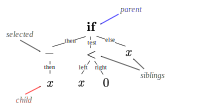
\includegraphics[scale=1.5]{src/image/position-tree.pdf}
%  \end{center}
%  
%  \caption{A simple expression as an AST, annotated to show relative node positions.}
%  \label{fig-position-tree}
%\end{figure}

\begin{figure}
  \begin{center}
  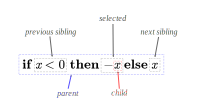
\includegraphics[scale=1.5]{src/image/position-ann.pdf}
  \end{center}
  
  \caption{A simple expression in \Meta, annotated to show relative node positions.}
  \label{fig-position}
\end{figure}


\subsection{Edit Actions}
The editor provides a range of operations on source nodes, which the user can use to construct and modify node trees. The examples in the next chapter will show them in action. 
%The current prototype provides only basic editing operations; to demonstrate a truly usable system would involve more investment in making common operations intuitive and efficient. Edit actions may be invoked through menus or keystrokes. 

There are just two primitive operations.

\emp{Delete} removes the selected node from its parent. If the parent is a map, it will no longer have any value for the attribute that was occupied by the selected node. If a sequence, the node is removed and any following children move to smaller indices. Note that a simple delete removes an entire subtree, not just the selected node itself.

\emp{Insert} adds a new node as a child of the selected node with a particular attribute name or index. If the selected node is a map, any previous child with the same attribute name is replaced. If a sequence, the new child pushes any existing children to the right.

All other edits are composed out of those two primitives:

\emp{Replace} deletes the selected node and inserts a new node in the same position.

\emp{Swap with previous} exchanges the places of the selected node and the previous sibling, by a sequence of three replace operations. \emp{Swap with next} is similar.

\emp{Insert parent} Interposes a new node between the selected node and its parent, by deleting the selected node, constructing a new node with it as a child, and then inserting the new node in the same position.

%\temp{Change type?}

%\temp{Swap with parent?}

\emp{Copy} does not affect the selected node, but saves a reference to it as a separate piece of editor state (the \emp{clipboard}).

\emp{Cut} copies and then deletes the selected node.

\emp{Paste} replaces the selected node with the contents of the clipboard.

When a new node is to be introduced, a simple interface is presented to allow the node's type to be specified. Another UI allows primitive values to be edited.

Before each edit operation, the current source AST and the identity of the selected node are pushed onto a stack of previous states. When the \emp{undo} action is performed, the most recent state is popped from the stack and restored. Because each edit involves $O(\log n)$ nodes, this is efficient enough for extended use.

When any editing action changes the source AST, the editor re-reduces the entire program and then redisplays the new reduced target tree. When a grammar is edited, the grammar itself is re-displayed, and then any reductions that were compiled from it are regenerated and any programs using them are redisplayed as well. This environment allows languages to be redefined dynamically.

%\subsection{Errors \todo{}}

